
\begin{figure}
\center

	\begin{subfigure}[t]{0.22\textwidth}
		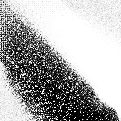
\includegraphics[width=\textwidth]{images/findings/experiments/punishment/strategies_handmaxmin.png}
		\caption{\handmaxmin}
	\end{subfigure}
	~
	\begin{subfigure}[t]{0.22\textwidth}
		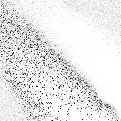
\includegraphics[width=\textwidth]{images/findings/experiments/punishment/strategies_handmaxavg.png}
		\caption{\handmaxavg}
	\end{subfigure}
	~
	\begin{subfigure}[t]{0.22\textwidth}
		
\includegraphics[width=\textwidth]{images/findings/experiments/punishment/strategies_handmaxmed.png}
		\caption{\handmaxmed}
	\end{subfigure}
	~
	\begin{subfigure}[t]{0.22\textwidth}
		
\includegraphics[width=\textwidth]{images/findings/experiments/punishment/strategies_handmaxposs.png}
		\caption{\handmaxposs}
	\end{subfigure}

	\begin{subfigure}[t]{0.22\textwidth}
		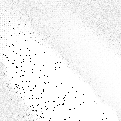
\includegraphics[width=\textwidth]{images/findings/experiments/punishment/strategies_cribminavg.png}
		\caption{\cribminavg}
	\end{subfigure}
	~
	\begin{subfigure}[t]{0.22\textwidth}
		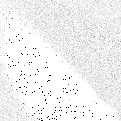
\includegraphics[width=\textwidth]{images/findings/experiments/punishment/strategies_peggingmaxavggained.png}
		\caption{\peggingmaxavggained}
	\end{subfigure}
	~
	\begin{subfigure}[t]{0.22\textwidth}
		
\includegraphics[width=\textwidth]{images/findings/experiments/punishment/strategies_peggingmaxmedgained.png}
		\caption{\peggingmaxmedgained}
	\end{subfigure}
	~
	\begin{subfigure}[t]{0.22\textwidth}
		
\includegraphics[width=\textwidth]{images/findings/experiments/punishment/strategies_peggingminavggiven.png}
		\caption{\peggingminavggiven}
	\end{subfigure}

\caption{
	Final strategy graphs for an agent which has less severe punishment
	after training for one million games.
}
\label{fig:findings-expts-punish-strats}
\end{figure}
